\chapter{Transit Spectra}
\label{spectra}
Exoplanet transits have become the most consistent means of detecting
 exoplanets, and exoplanet transit spectra has become the most common method of
 analyzing an exoplanet's atmosphere. Before the launch of JWST, quality
 spectra have been difficult to produce and is often limited to visible wavelengths. The
 most observable planets for exoplanet spectra are hot Jupiters because they will have
 a large atmosphere and large transit depths, and even in those cases,
 Earth-based telescopes have had low signal to noise and spectral resolution.
 Recent observational work including \citet{essenwasp33b} and
 \citet{ducrottrappistspectra} have shown promising results, but have also shown
 that before the launch of JWST, models and theory are far ahead of
 observations. Using the PSG, we will be able to see spectra that is at James
 Webb's maximum resolution without noise, which will enable us to explore
 spectra and analyze
 it in ways that will not be observationally possible even after JWST
 launches.

The PSG can return spectra for a variety of JWST instruments, including
 MIRI-MRS (mid infrared, medium resolution), MIRI-LRS (mid infrared, low
 resolution), NIRSpec 2700 (near infrared, medium resolution), and NIRSpec 1000
 (near infrared, low resolution). The range of wavelengths that can be measured
 range from $\SI{1}{\micro\meter}$ to $\SI{28}{\micro\meter}$. The shorter
 wavelengths are usually referred to as the near infrared, which can sometimes
 be viewed from ground based telescopes. The longer wavelengths are in the
 mid-infrared, and are sometimes called the thermal infrared because while the
 near infrared features mostly absorption and emission features of molecules,
 the longer wavelengths are dominated by blackbody radiation of cool objects.

Transit spectroscopy's primary strength is its ability to detect atmospheric
 species, and the shorter wavelengths will produce the most significant results.
 In Chapter \ref{thermalphasecurves}, I will show that beyond
 $\SI{17}{\micro\meter}$, the thermal
 emission of an exoplanet dominates over absorption features.

In a noiseless spectra, it is often convenient to show as much information as
 possible, which can be done by combining the NIRSpec and MIRI instruments to
 produce a single spectra. This result for $\SI{1}{\bar}$ \chem{CO_2} and
 $\SI{0.4}{\bar}$ \chem{N_2}
 is shown in Figure \ref{nirspecmiri}. Over a small range around
 $\SI{5}{\micro\meter}$, the two overlap. The axis are scaled logarithmically to
 emphasize the shorter wavelengths as they will generally have better signal to
 noise. The signals are reported in parts per million, relative to the star. A
 series of features can be easily identified, the most obvious of which
 is the $\SI{15}{\micro\meter}$ spike caused by \chem{CO_2}. Some of the features
 are due to \chem{H_2O}, but few to no features are due to \chem{N_2} because
 it does not absorb in the infrared. However, collisional processes involving
 \chem{N_2} can cause absorption \citep{badhan19}, but this is generally
 overwhelmed by \chem{CO_2} and \chem{H_2O} absorption features.

\begin{figure}[ht]
    \begin{center}
        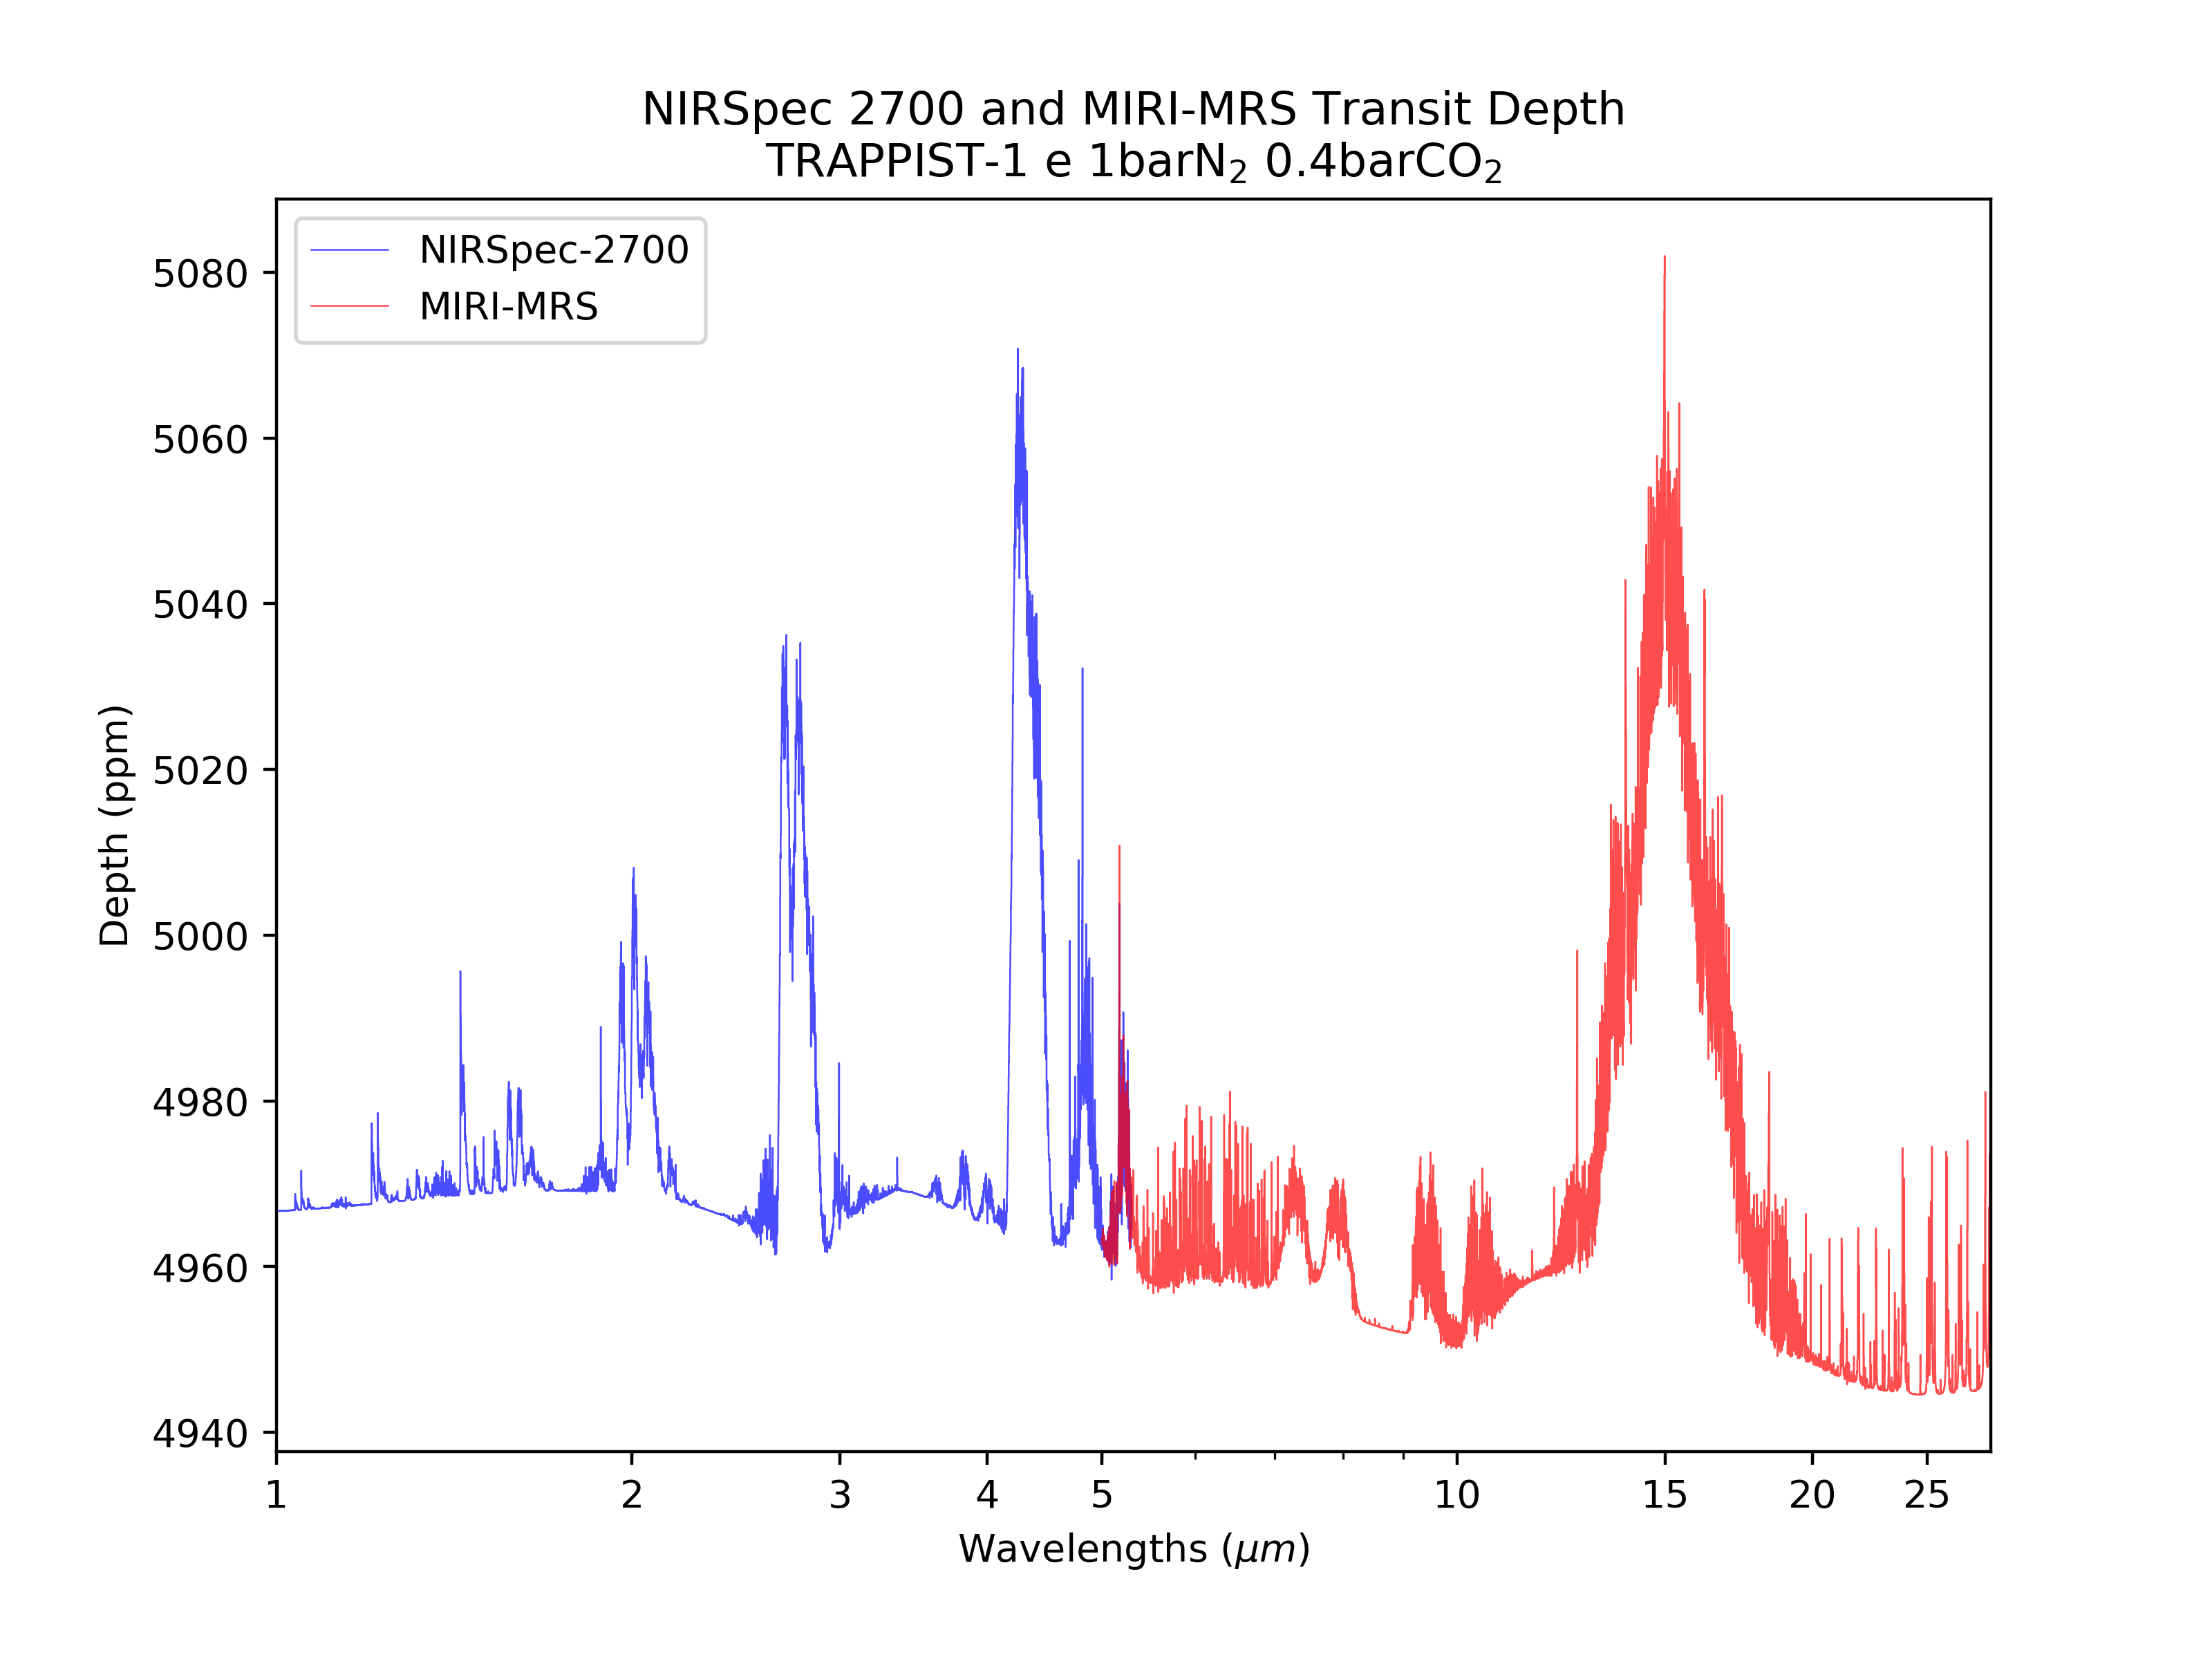
\includegraphics[width=\textwidth]{spectra/miri_nirspec_depth.png}
        \caption[Transit spectra of NIRSpec-2700 and MIRI-MRS]{Transit spectra
         of NIRSpec-2700 and MIRI-MRS. In this spectra, there are a number of
         interesting absorption features. The widest feature is the $\SI{15}{\micro\meter}$
         \chem{CO_2} absorption, which is both the widest and highest feature.
         Another distinguished feature is the $\SI{6}{\micro\meter}$ series of thin lines, which
         is due to \chem{H_2O}. The logarithmic axis showed a more balanced
         spectra showing both the NIRSpec and MIRI instruments. Otherwise, the
         spectra would be dominated entirely by MIRI.}
        \label{nirspecmiri}
    \end{center}
\end{figure}

For exoplanet transit spectra, the vertical axis is called transit depth, but
 it is slightly different than the transit depth $D$ discussed previously. It is
 a spectral transit depth, $D(\lambda)$. Instead of describing the size of the
 planet and atmosphere, it describes the size of the planet and atmosphere at
 a specific wavelength. $D(\lambda)$ based on the atmospheric species
 that absorb at that wavelength. The $\SI{15}{\micro\meter}$ spike would
 indicate that the
 atmosphere is effectively larger at that wavelength due to \chem{CO_2}, and
 therefore less
 of TRAPPIST-1's light will make it to the telescope. In effect, $D(\lambda)$
 indicates absorption, and the cause of this dip will indicate composition.
 In general, these spectral lines would be compared to a list of spectral lines
 measured in a lab. We can skip this step with the PSG and by modifying the
 input atmosphere profile. Instead of sending the standard profile to the PSG,
 modified atmosphere profiles can be created, which can then be compared to the standard
 outputs. For example, to determine which features are due to \chem{H_2O}, the
 PSG pipeline can be rerun, but with the \chem{H_2O} abundance artificially
 set to zero (including
 the liquid and ice clouds). The outputs from the PSG can then be compared, and
 the difference between the two spectra is the effective contribution of
 \chem{H_2O}. This procedure can be done for \chem{CO_2}, \chem{H_2O}, and
 \chem{N_2}, all of which are shown together in Figure \ref{nospecies}.
 Additionally, this plot demonstrates the validity of adding additional layers to
 the atmospheric profile as was discussed in Chapter \ref{models}, one of the
 most significant assumptions made in the creation of this
 spectra. In this figure, the spectra without the additional layers has an
 artificial ceiling around $\SI{15}{\micro\meter}$ because the PSG found the atmosphere to be
 completely opaque in those wavelengths. Adding the additional layers shows a
 stronger signal because the atmosphere continues to be opaque at pressures much
 below $\SI{1}{\milli\bar}$.

 \begin{figure}[ht]
    \begin{center}
        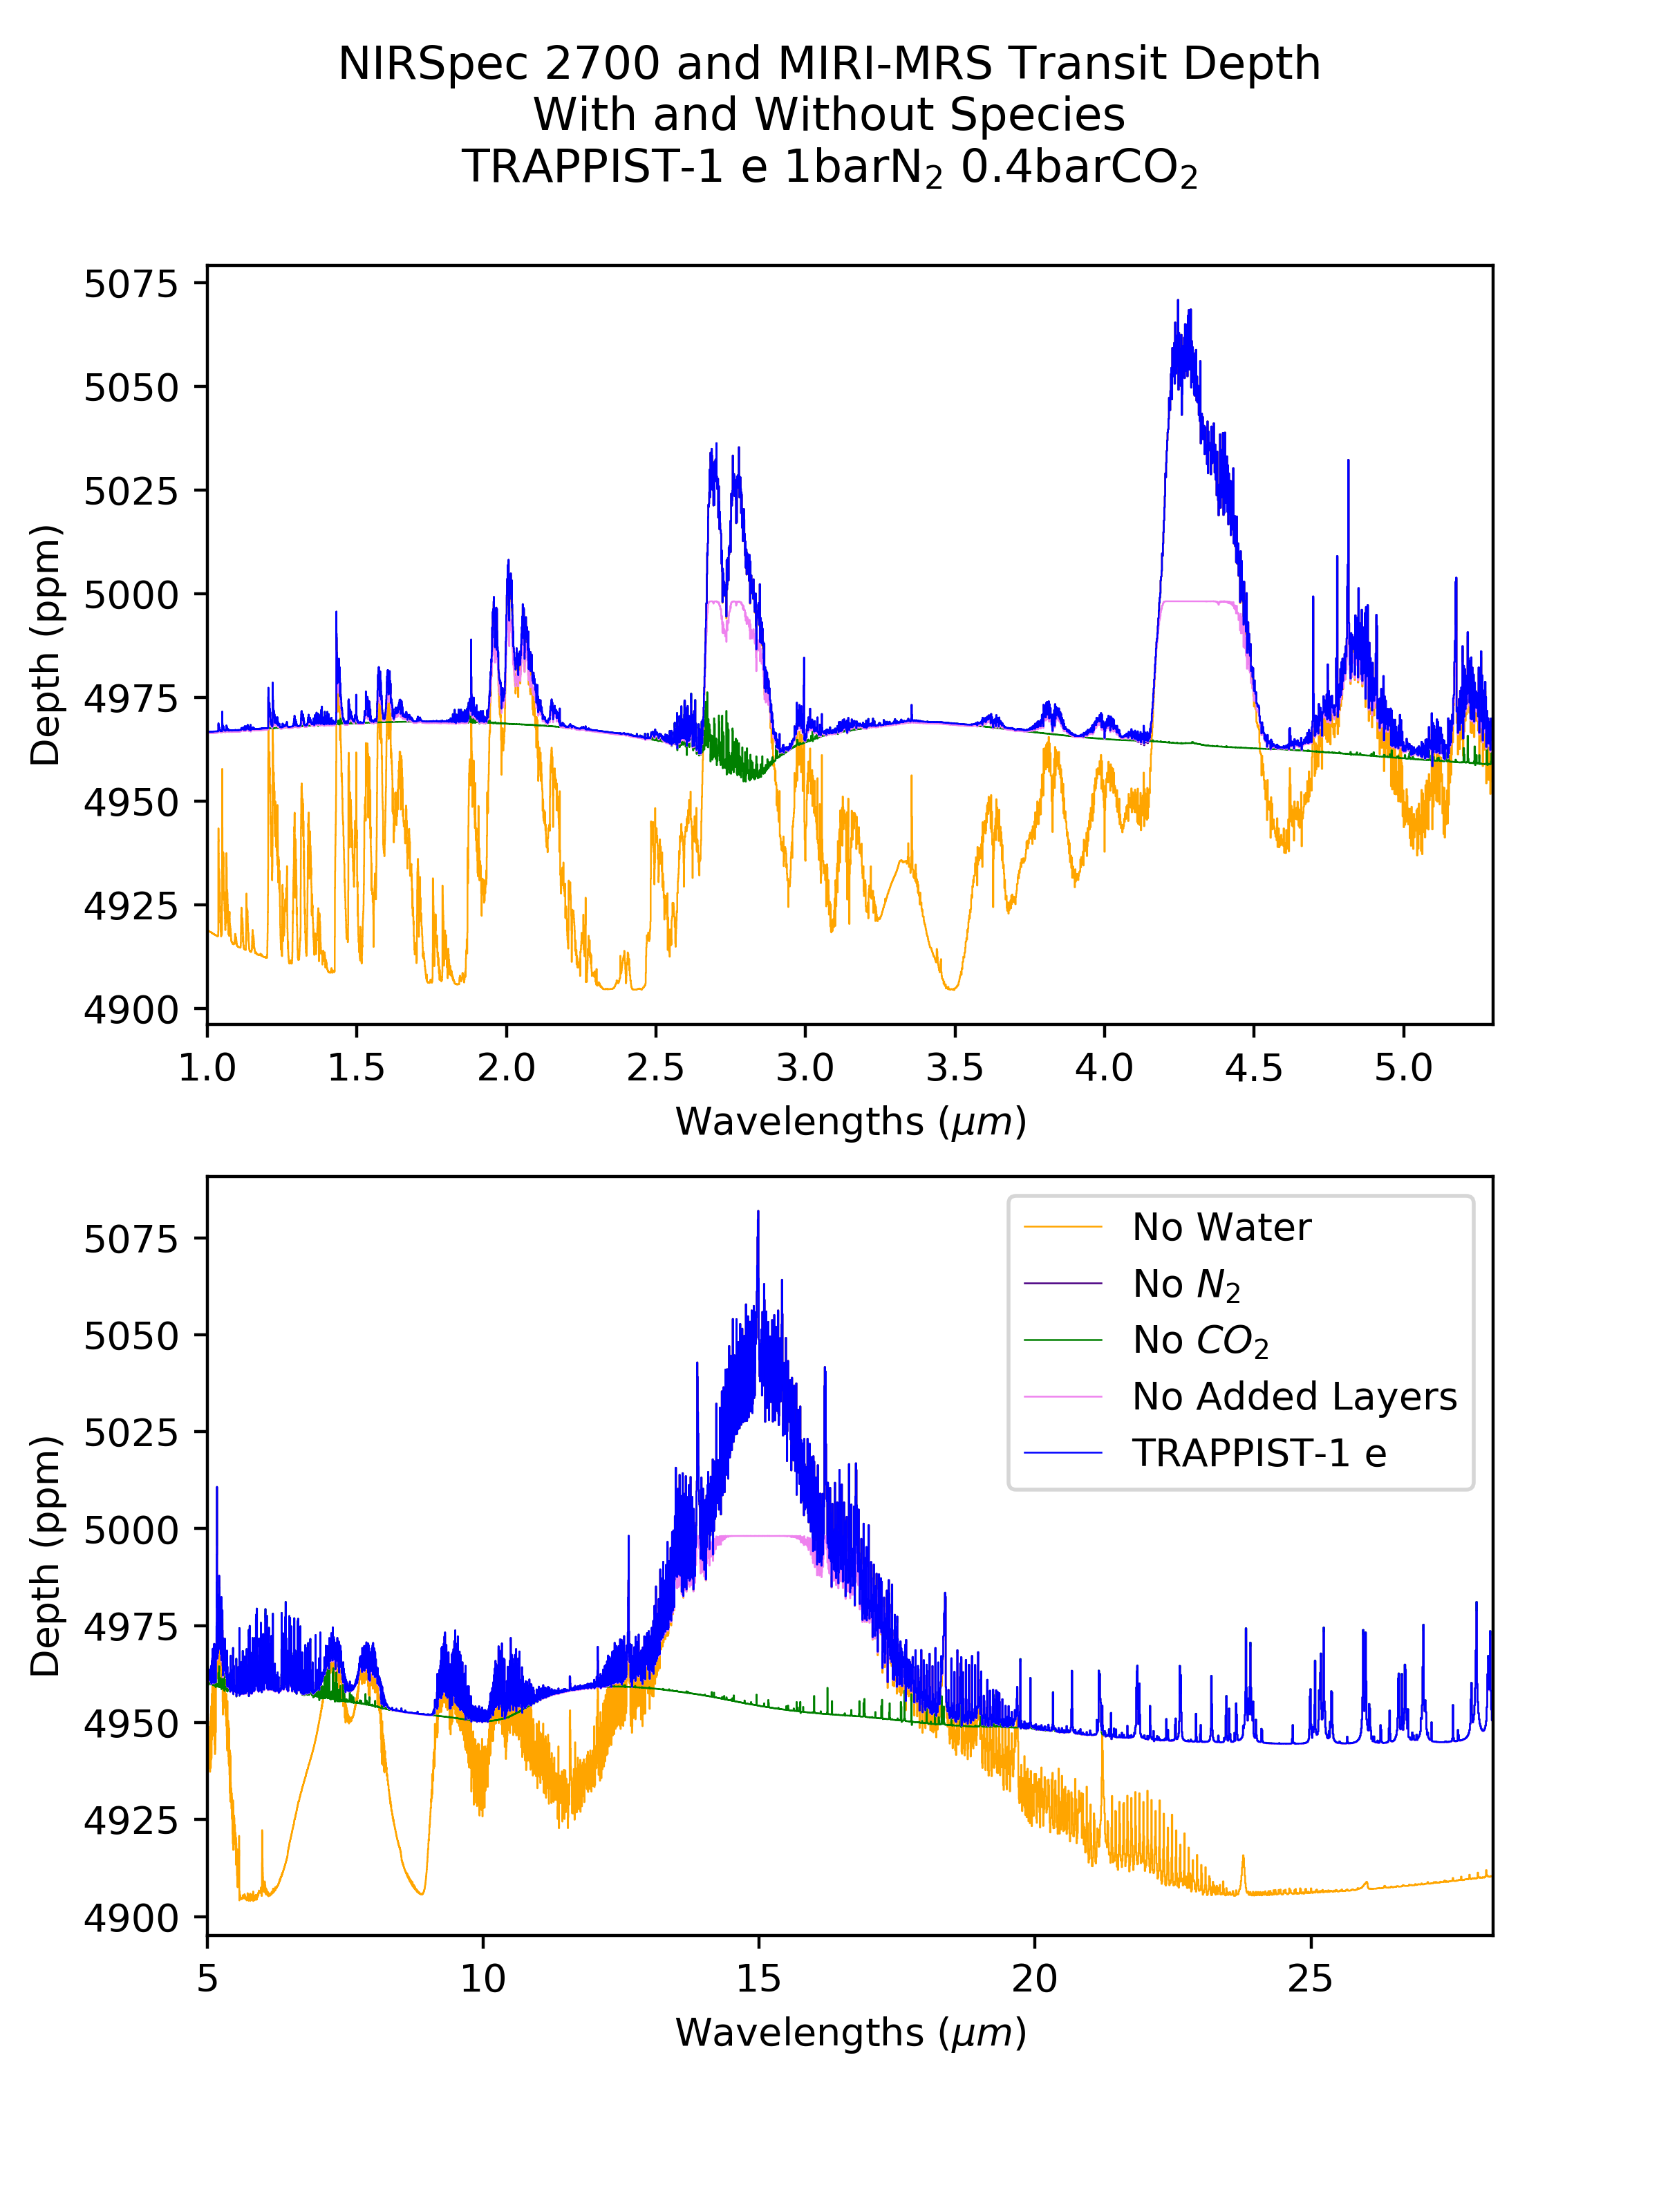
\includegraphics[width=0.8\textwidth]{spectra/nirmiri_without_species.png}
        \caption[Transit Spectra Without Species]{Transit
         Spectra Without Species. The top diagram is the NIRSpec transit and the
         bottom is the MIRI transit. Each color represents a different
         PSG simulation, where a different atmospheric species was zeroed-out
         before being sent to the PSG. The models are plotted in reverse order
         of the legend, with the normal transit on the top. The model without
         \chem{N_2} completely overlaps the blue plot because \chem{N_2} doesn't
         absorb in
         the infrared. Others only absorb at specific wavelengths, which is
         where the colors are visible.}
        \label{nospecies}
    \end{center}
\end{figure}

From Figure \ref{nospecies}, it is clear that the wavelengths between
 $\SI{12}{\micro\meter}$ and $\SI{18}{\micro\meter}$ are almost completely
 dominated by \chem{CO_2}, but it is
 surrounded on all sides by various \chem{H_2O} features, the strongest of
 which is at $\SI{6}{\micro\meter}$. It is in diagrams like this where the
 absence of other
 atmospheric species is most noticeable. \chem{O_3} would produce a large
 spike at $\SI{9}{\micro\meter}$, as well as other areas. The addition of many
 species would
 make the spectra more complex and more realistic.

Several of these larger features would be more easily detectable, even when MIRI
 is used in a low-resolution configuration. The features stand out primarily
 because they are wide as well as deep, and both are essential for strong signal
 to noise. The question then becomes ``how strong is this signal and can it be
 used to detect \chem{H_2O} from Earth?'' Before we can consider analyzing
 signal to noise ratios, we must first create a method of measuring these
 variances that we can see in Figure \ref{nospecies}.

For an example, we will focus on measuring the \chem{CO_2} in the MIRI spectra.
 Using the values from Figure \ref{nospecies}, we can define a subset of
 the total wavelength range of MIRI where \chem{CO_2} is significant. We can
 define this region using the condition
 $D(\lambda) - D(\lambda)_{\mathrm{No\ \chem{CO_2}}} \geq 5\,\mathrm{ppm}$. Any
 wavelength that matches this condition will be considered a significant
 wavelength for
 \chem{CO_2}, and will be notated as $\lambda_\chem{CO_2}$. In order to use
 this wavelength subset, we should no longer use
 the PSG's output in units of transit depth, we must now use it in a more
 ``raw'' unit of spectral intensity,
 \si{\watt\per\meter^2\per\steradian\per\micro\meter}.
 In this case, we will measure the quantity $\Delta F(\lambda)=F(\lambda)_
 \mathrm{pre\ transit} - F(\lambda)_\mathrm{transit}$. With signals in units of
 spectral intensity, we can more easily perform complex analysis on the signals.
 Using this subset, the signals can be summed using the equation

\begin{equation}
    \bar{D}_\chem{CO_2} = \frac{\sum_{\lambda_\chem{CO_2}}
    \Delta F(\lambda_\chem{CO_2})}
    {\sum_{\lambda_\chem{CO_2}} F(\lambda)_\mathrm{pre\ transit}},
    \label{reductionfunction}
\end{equation}
where $\bar{D}_\chem{CO_2}$ is the average transit depth over the range of
 wavelengths where \chem{CO_2} is significant. The underlying
 goal of this method is to improve the overall signal to noise by summing across
 wavelengths. Very little information is lost using this method. Although
 ``micro-features'' in the spectra will disappear, this isn't an issue because
 they were already immeasurable due to the high noise.

With a solidly defined technique for measuring a signal, $\bar{D}_\chem{CO_2}$,
 we must now consider how the noise will be affected by this calculation. The
 noise results returned by the PSG don't consider some sources of noise. Other
 softwares like PandExo incorporate more sources of noise \citep{batalha17}, but
 the results returned by the PSG are still useful as they provide a lower limit
 on the noise. The noise before and during the transit will be similar to the
 point that they are indistinguishable, so a single noise function $N(\lambda)$
 will be used to describe all measurements. Noise is also a function of exposure
 count and exposure time. The values used here will be the noise for a single
 transit, but the error should decrease from this according to the rule
 $N(\lambda)\propto 1/\sqrt{t}$ where $t$ is the exposure time. In order to
 compute the error in $\bar{D}_\chem{CO_2}$, we need to go through step by step.
 The numerator uses subtraction, and the errors are the same magnitude, so the
 numerator's
 error is simply root two the original error. For the fraction, the numerator is
 much smaller than the denominator, and their errors are of similar magnitude,
 so the
 fractional error is approximately the fractional error in the numerator. The
 error in $\bar{D}_\chem{CO_2}$ is therefore given by the equation

\begin{equation}
    \delta\bar{D}_\chem{CO_2}
    =\bar{D}_\chem{CO_2}\left|\frac{\sqrt{2}\delta F(\lambda)}{F(\lambda)}\right|,
\end{equation}
where the absolute value implies adding each wavelength bin in quadrature, hence
 resolving the dependence on wavelength.

$\bar{D}_\chem{CO_2}$ and $\bar{D}_\chem{H_2O}$ are directly observable values,
 and similar values could be computed for other species like \chem{CH_4} and
 \chem{O_3} if future models can incorporate them. $\bar{D}$ is an interesting
 measurement, but a question remains, what can it tell us about an exoplanet?
 To determine this, the ensemble of climate models must be used, and their
 values for $\bar{D}$ cross-referenced. As to how to might impact the value,
 the answer is non-trivial. It is certainly possible that surface temperature,
 surface pressure, partial pressures of the relevant species, or any number of
 other factors could be significant. The ensemble of climate models have
 different values for all these parameters, and they can be cross-referenced
 with the computed values of $\bar{D}$, to determine which values are
 significant. The simplest method of determining correlation is using the $r^2$
 method, which will be used in this case. Table \ref{rsquared} computes the
 significance of different atmospheric parameters on $\bar{D}$. The only
 parameter strongly correlated with $\bar{D}$ is the surface temperature. All
 other parameters prove insignificant. Surprisingly, $\bar{D}_\chem{CO_2}$
 proves unreliable at measuring the partial pressure of \chem{CO_2}. These
 results match the simple prediction that the most significant attribute in the
 transit depth is the overall height of the atmosphere. A high surface
 temperature will
 produce a high atmospheric scale height, which will lead to a larger transit
 depth. Unfortunately, it means that simply measuring $\bar{D}$ is not an
 effective method of identifying the abundance of certain species in an
 atmosphere. Although the presence of a feature like a spike at
 $\SI{15}{micrometer}$ would
 indicate the presence of \chem{CO_2}, it alone cannot be used to measure
 the abundance.

\begin{table}[htbp]
    \begin{center}
        \begin{tabular}{lllr}\hline
        Parameter & Instrument & Species Measured & $r^2$\\\hline
        \multirow{4}{*}{Surface Temperature}
        &\multirow{2}{*}{NIRSpec}
        &\chem{CO_2} & 0.834\\
        &&\chem{H_2O}& 0.757\\
        &\multirow{2}{*}{MIRI}&\chem{CO_2} & 0.881\\
        &&\chem{H_2O}& 0.821\\
\hline
        \multirow{4}{*}{Surface Pressure} &\multirow{2}{*}{NIRSpec}
        &\chem{CO_2} & 0.496\\
        &&\chem{H_2O}& 0.593\\
        &\multirow{2}{*}{MIRI}&\chem{CO_2} & 0.563\\
        &&\chem{H_2O}& 0.650\\
\hline
        \multirow{4}{*}{\chem{N_2} Partial Pressure}
        &\multirow{2}{*}{NIRSpec}
        &\chem{CO_2} & 0.415\\
        &&\chem{H_2O}& 0.501\\
        &\multirow{2}{*}{MIRI}&\chem{CO_2} & 0.456\\
        &&\chem{H_2O}& 0.528\\
\hline
        \multirow{4}{*}{\chem{CO_2} Partial Pressure}
        &\multirow{2}{*}{NIRSpec}
        &\chem{CO_2} & 0.036\\
        &&\chem{H_2O}& 0.034\\
        &\multirow{2}{*}{MIRI}&\chem{CO_2} & 0.060\\
        &&\chem{H_2O}& 0.066\\\hline
        \end{tabular}
        \caption[Correlation Coefficients of Atmospheric Parameters and
        $\bar{D}$]{Correlation Coefficients of Atmospheric Parameters and
        $\bar{D}$. Some of the most scientifically significant planetary
        attributes are shown in the left column. Their contribution to the
        transit depth is shown in the right column, where a number close to 1
        indicates a strong correlation and a number close to 0 indicates a weak
        correlation. Both atmospheric species (implying a different set of
        wavelengths) and instrument will impact the transit depth, and 
        therefore produce different $r^2$ values. Surface temperature has a
        strong correlation to the transit depth for both \chem{CO_2} and
        \chem{H_2O}, but all others have weak or no correlation.}
        \label{rsquared}
    \end{center}
\end{table}

The relationship between surface temperature and $\bar{D}$ can be visually seen
 in Figure \ref{depthfromtemp}. In this case, the $1\sigma$ noise after 10
 transits is shown. Often NIRSpec produces lower noise, and \chem{H_2O} produces
 stronger signals because it is present in more wavelengths across the spectrum.
 These results show errors low enough, that one could reasonably back out a
 surface temperature if given a value for $\bar{D}$.
 Unfortunately, as suggested in Table \ref{rsquared}, no similar graphs could
 be produced for dependences on other atmospheric parameters.

\begin{figure}[ht]
    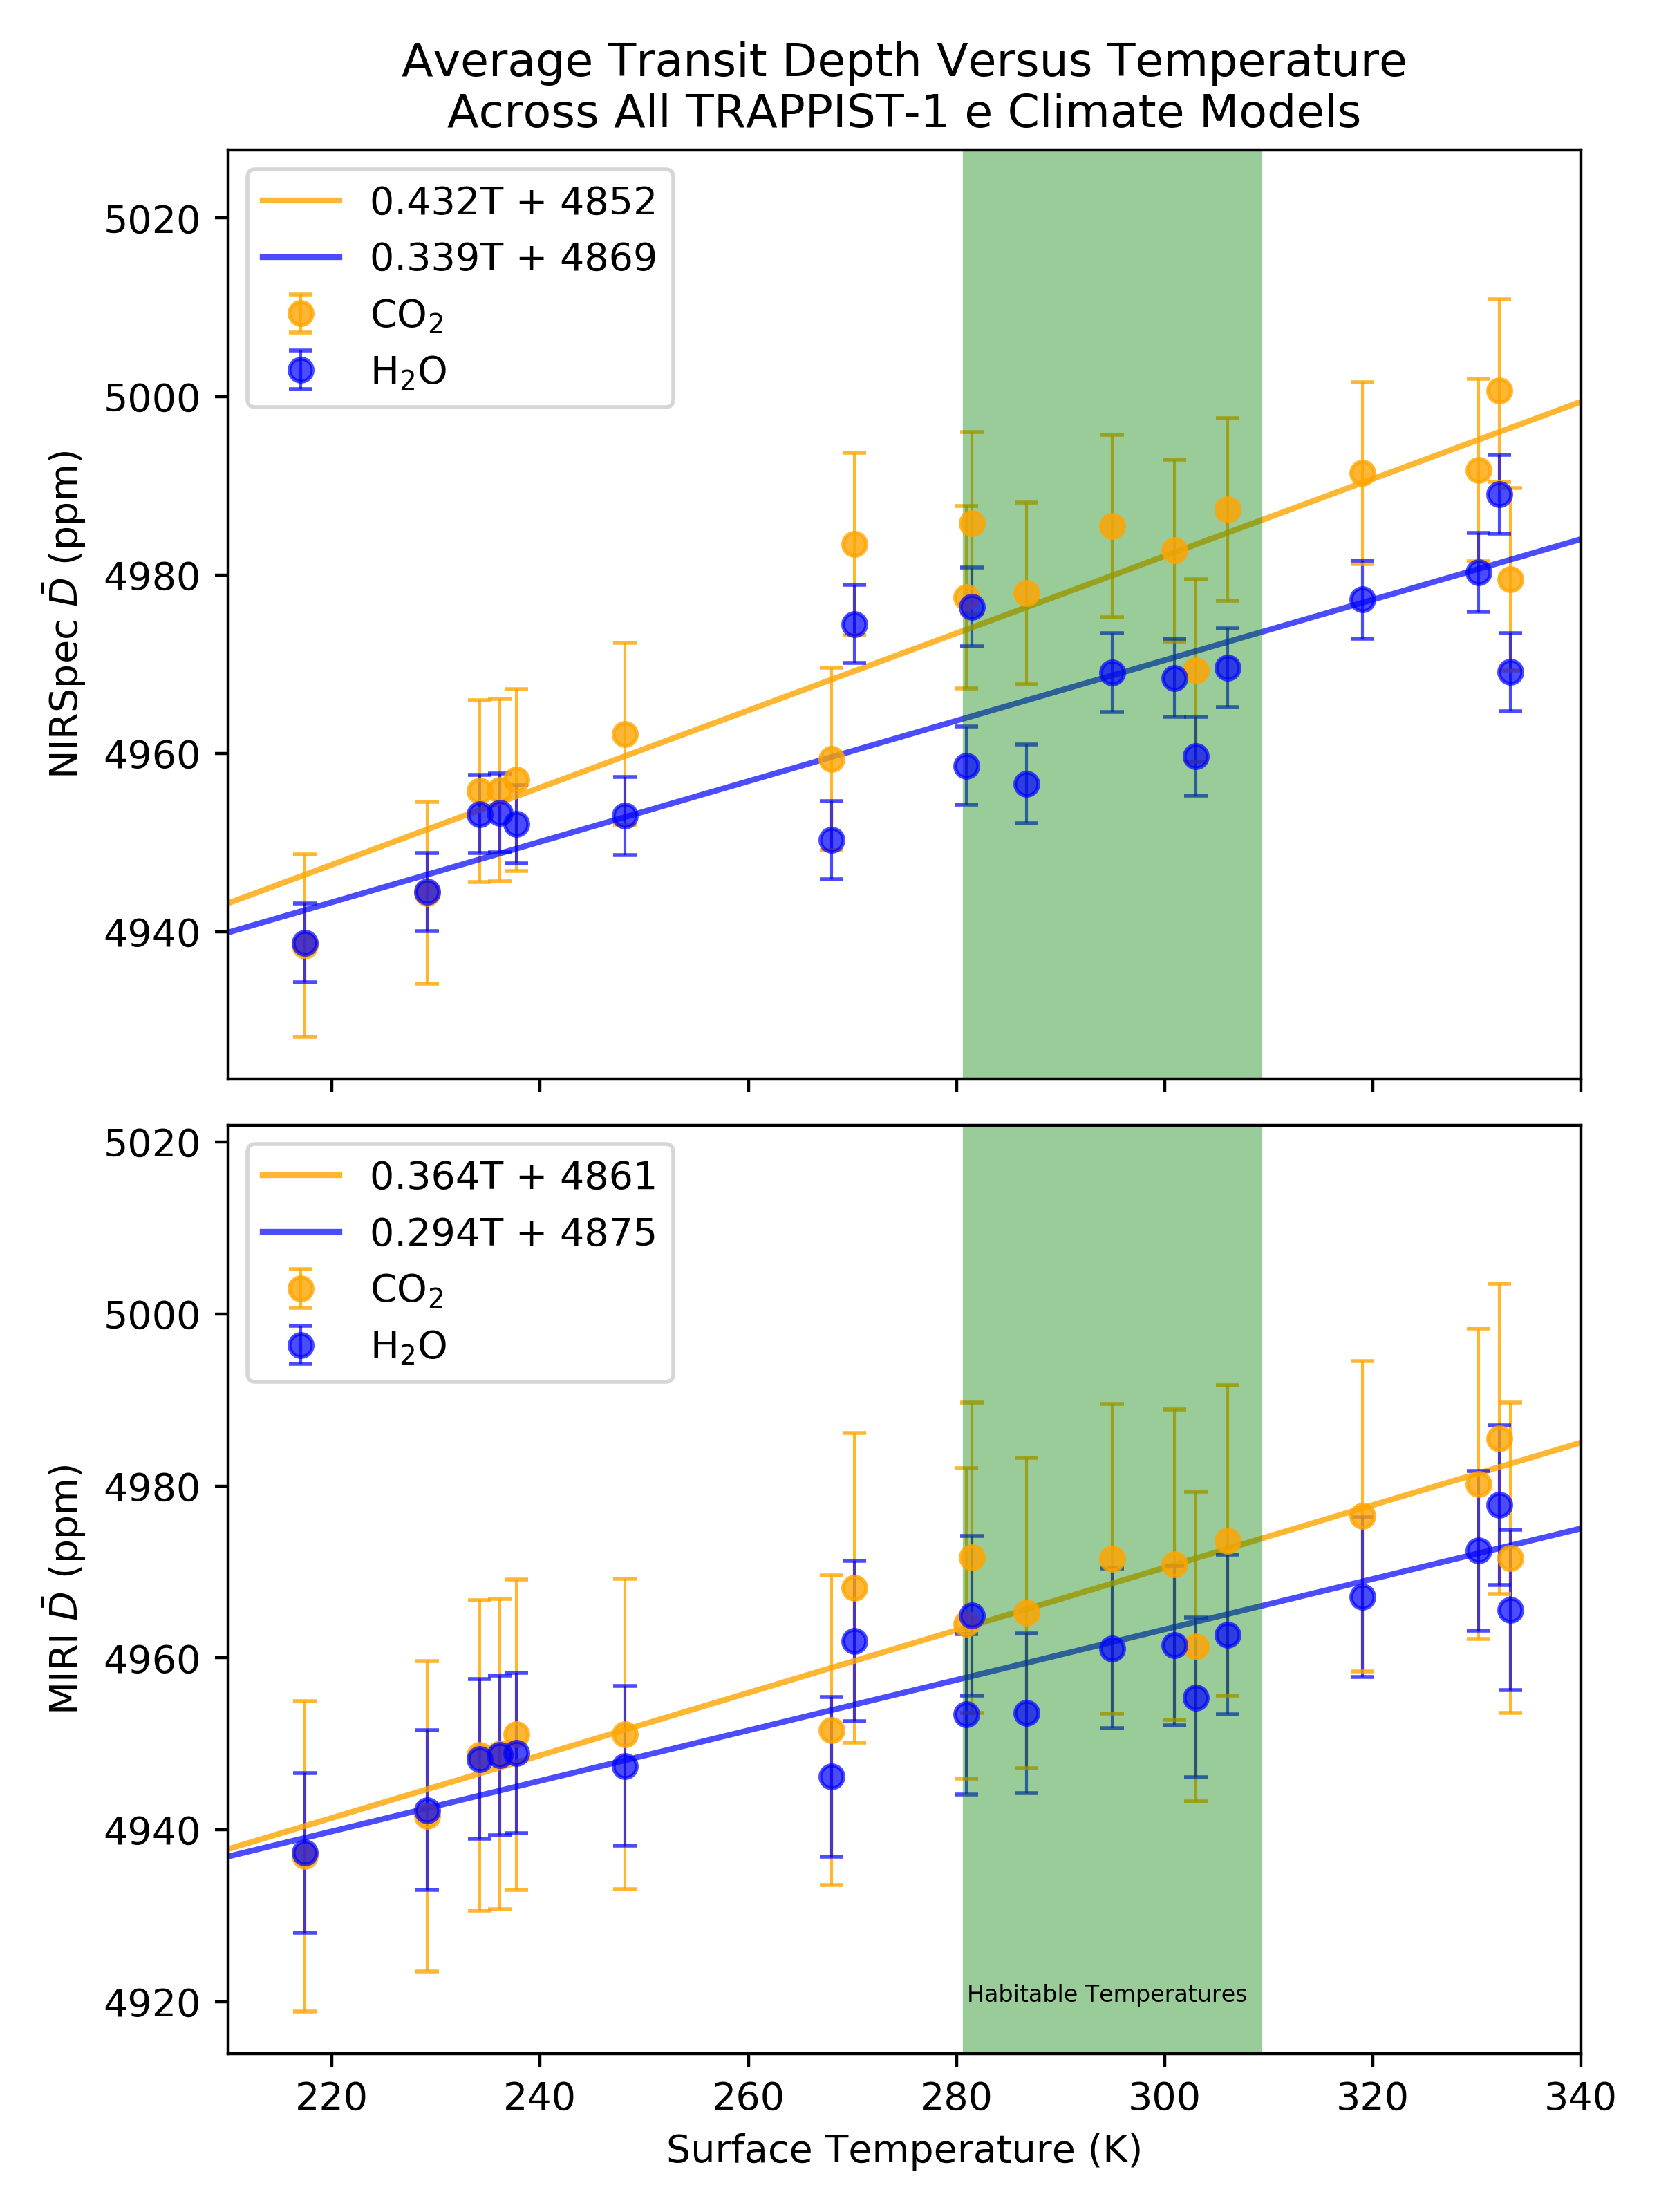
\includegraphics[width=0.8\textwidth]{./spectra/depth_from_temp.png}
    \caption[Transit Depth Versus Surface Temperature]{Transit Depth Versus
    Surface Temperature. Blue points are measurements of
    $\bar{D}_\chem{H_2O}$, red points are measurements of $\bar{D}_\chem{CO_2}$.
    Given the error bars on these points, it is hard to justify anything more
    than a linear fit between temperature and $\bar{D}$. Across both
    instruments, \chem{CO_2} has a steeper slope than \chem{H_2O}, implying that
    it would be a better wavelength range to use when trying to determine
    surface temperature.}
    \label{depthfromtemp}
\end{figure}

For the wavelengths used to measure $\bar{D}_\chem{CO_2}$ in MIRI, the $1\sigma$
 error found by the PSG is 85.8 ppm after 1 transit. It is worth noting that
 since the PSG
 likely underestimates the total noise, the error is even larger.
 Even the most prominent features in the spectra are only ~100 ppm tall. Some
 features like $\SI{15}{micrometer}$
 \chem{CO_2} and $\SI{6}{micrometer}$ \chem{H_2O} produce approximately 100 ppm
 gaps, as shown
 in Figure \ref{nospecies}, but those signals are only that large for a few
 wavelengths, and the values of $\bar{D}$ would produce lower values, with
 better signal to noise. Overall, this is producing a rather bleak picture for
 detecting atmospheric parameters such as partial pressures of species or
 surface pressure. However, it is possible that when JWST launches,
 observed spectra can be compared with these model results to produce more
 accurate conclusions. Even though some measurements of $\bar{D}$ proved weak
 across models, they produced strong signals relative to the same models with
 missing atmospheric species. When JWST launches and spectra is actually
 collected, these techniques which can now only be tested on models will likely
 prove to be useful first steps in observation analysis.
